\subsection{Active Armrest}
\begin{figure}[h]
\centering
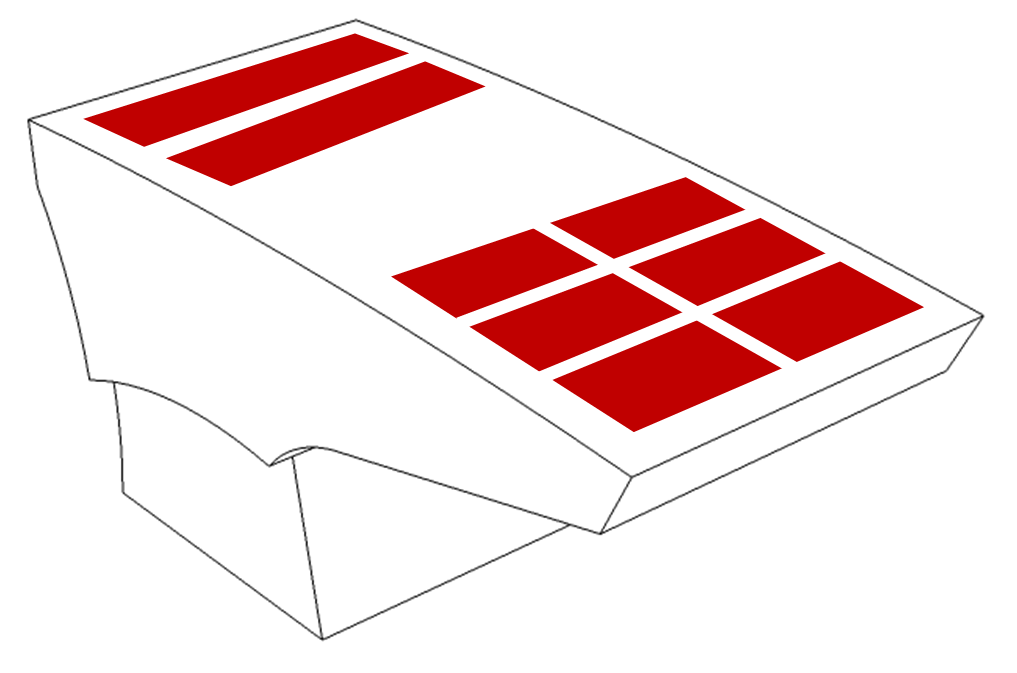
\includegraphics[width=0.4\textwidth]{images/active_armrest}
\caption{Active armrest sketch - six electrodes for finger gesture detection in front, two for arm detection in back}
\label{fig:armrest_sketch}
\end{figure}
The Active Armrest is a prototype to demonstrate unobtrusive gestural interaction in the domain of automotive applications [74]. The interior of modern cars can be considered a smart environment as it includes an ensemble of sensors and actors that adapt the system behavior according to user preference.
 
%Figure 24 Active armrest sketch - six electrodes for finger gesture detection in front, two for arm detection in back
Many cars use touch screens or jog dials to control primary and secondary car functions \cite{schmidt2010automotive}. Capacitive proximity sensors allow integrating interactive areas into different existing surfaces of a car, e.g. an armrest. The Active Armrest is using a set of eight sensors that are separated into two different groups. There are two larger electrodes in the back of the armrest that are dedicated to recognizing the presence of an arm. In the front of the armrest there is an array of six small electrode sensors, in order to register finger gestures, as shown in Figure \ref{fig:armrest_sketch}. The basic idea is to disallow interaction when the arm is resting and enable it once it's lifted. The Active Armrest supports swiping gestures of a single finger and static holding gestures of two fingers. This allows controlling various typical automotive applications, e.g. a navigation application, whereas holding is zooming in and out and swipe pan through the maps. Similar applications, such as multimedia features and comfort settings can be controlled in a similar fashion.

